\chapter{Системы со связями и гамильтоново движение}

\lectureoverview{Две системы со связями показывают, почему механика Лагранжа настолько эффективна: как только выбраны подходящие координаты, уравнения движения и соответствующие законы сохранения следуют без явного вычисления сил связи. Эти же примеры затем подводят к гамильтоновой механике, в которой координаты и импульсы образуют фазовое пространство, гармонический осциллятор превращается в жёсткое вращение, а два уравнения Гамильтона первого порядка заменяют каждое уравнение Эйлера--Лагранжа второго порядка.}

\section{Что значит решить механическую задачу}

Непосредственная цель метода Лагранжа — практическая. Клин, скользящий по полу, и двойной маятник можно рассматривать и с помощью законов Ньютона, но неизвестные силы контакта и натяжения быстро делают вычислительный учёт громоздким. Когда правила механики Лагранжа уже известны, те же задачи сводятся к последовательности чётко определённых шагов:
\begin{enumerate}
  \item выбрать независимые координаты, задающие мгновенную конфигурацию;
  \item выразить кинетическую и потенциальную энергии через эти координаты;
  \item составить \(L=T-V\) и применить уравнения Эйлера--Лагранжа.
\end{enumerate}

Для наших целей задача уже \emph{решена}, когда её уравнения движения записаны правильно. Можно по-прежнему хотеть получить траекторию в замкнутой форме, но это уже отдельный вопрос. Нелинейные дифференциальные уравнения можно интегрировать численно, как только механическая постановка завершена. Трудная часть часто состоит не в интегрировании; она состоит в том, чтобы найти переменные, которые учитывают связи, не вводя избыточных неизвестных сил.

\section{Частица, скользящая по движущемуся клину}

Рассмотрим клин массы \(M\), которому разрешено без трения скользить вдоль горизонтальной плоскости. Точечная частица массы \(m\) обязана оставаться на наклонной грани. Здесь две степени свободы: одна задаёт положение клина, а другая — положение частицы на клине.

Пусть
\begin{equation}
  \begin{aligned}
    X&=\text{horizontal position of the wedge corner},\\
    x&=\text{horizontal displacement of the particle}\\[-0.2em]
     &\phantom{={}}\text{from that corner}.
  \end{aligned}
  \label{eq:l6-wedge-coordinates}
\end{equation}
Тогда абсолютная горизонтальная координата частицы равна \(X+x\). Этот выбор не единственный. Вместо него можно было бы использовать расстояние вдоль наклонной плоскости или абсолютную горизонтальную координату частицы. Допустима любая неизбыточная пара, задающая те же конфигурации, хотя одни пары выявляют структуру яснее, чем другие.

При фиксированном угле наклона \(\beta\) вертикальное смещение \(y\) не является независимой координатой:
\begin{equation}
  y=x\tan\beta,
  \qquad
  \dot y=\dot x\tan\beta.
  \label{eq:l6-wedge-constraint}
\end{equation}
Мы специализируемся на случае \(\beta=45^\circ\), так что \(y=x\) и
\(\dot y=\dot x\). Это упрощение убирает тригонометрические множители, не меняя сути примера.

\begin{figure}[htbp]
  \centering
  \includegraphics[width=0.84\textwidth]{lecture_06_figure_06.png}
  \caption{Движущийся клин, связанная частица и горизонтальная и вертикальная компоненты скорости, используемые в примере с \(45^\circ\).}
  \lectureframe{00:10:25}
\end{figure}

Кинетическая энергия клина равна
\begin{equation}
  T_{M}=\frac{M}{2}\dot X^2.
  \label{eq:l6-wedge-kinetic}
\end{equation}
Горизонтальная скорость частицы равна \(\dot X+\dot x\), а её вертикальная скорость — \(\dot x\). Поэтому её кинетическая энергия равна
\begin{equation}
  T_m=\frac{m}{2}\left[(\dot X+\dot x)^2+\dot x^2\right].
  \label{eq:l6-particle-kinetic}
\end{equation}
Выбрав нуль гравитационной потенциальной энергии при \(x=0\), получаем \(V=mgx\).
Следовательно,
\begin{equation}
  L=\frac{M}{2}\dot X^2
    +\frac{m}{2}\left[(\dot X+\dot x)^2+\dot x^2\right]
    -mgx.
  \label{eq:l6-wedge-lagrangian}
\end{equation}

\begin{figure}[htbp]
  \centering
  \includegraphics[width=0.86\textwidth]{lecture_06_figure_07.png}
  \caption{Геометрия клина, \(V=mgx\) и два вклада в кинетическую энергию, собранные на доске.}
  \lectureframe{00:14:15}
\end{figure}

\subsection{Канонический импульс определяется лагранжианом}

Канонические импульсы определяются лагранжианом, а не догадкой, основанной на скорости отдельной частицы:
\begin{align}
  p_X&=\frac{\partial L}{\partial\dot X}
      =M\dot X+m(\dot X+\dot x),
      \label{eq:l6-wedge-pX}\\
  p_x&=\frac{\partial L}{\partial\dot x}
      =m(\dot X+\dot x)+m\dot x.
      \label{eq:l6-wedge-px}
\end{align}
Первое выражение — это обычный полный горизонтальный импульс: клин даёт вклад \(M\dot X\), а частица даёт вклад
\(m(\dot X+\dot x)\). Здесь он появляется как импульс, сопряжённый координате \(X\).

\begin{figure}[htbp]
  \centering
  \includegraphics[width=0.86\textwidth]{lecture_06_figure_08.png}
  \caption{Канонические импульсы, сопряжённые координате клина \(X\) и относительной координате частицы \(x\).}
  \lectureframe{00:18:05}
\end{figure}

Лагранжиан не зависит явно от \(X\). Горизонтальный перенос всей установки действует как
\begin{equation}
  \delta X=\epsilon,
  \qquad
  \delta x=0.
  \label{eq:l6-wedge-translation}
\end{equation}
Общее правило для бесконечно малого преобразования симметрии
\begin{equation}
  \delta q_i=\epsilon f_i(q),
  \qquad
  Q=\sum_i p_i f_i
  \label{eq:l6-noether-rule}
\end{equation}
поэтому даёт \(Q=p_X\). Эквивалентно, \(X\) является циклической координатой, и
\begin{equation}
  \dot p_X=\frac{\partial L}{\partial X}=0.
  \label{eq:l6-wedge-conservation}
\end{equation}

Соответствующей симметрии вертикального переноса нет. Клин не может двигаться по вертикали, а изменение высоты частицы меняет гравитационную потенциальную энергию. Горизонтальный импульс сохраняется; вертикальный импульс этой подсистемы со связями — нет.

Для относительной координаты уравнение Эйлера--Лагранжа имеет вид
\begin{equation}
  \dot p_x=\frac{\partial L}{\partial x}=-mg.
  \label{eq:l6-wedge-force}
\end{equation}
Эта строка на доске потребовала исправления знака. Надёжный путь — начать с \(L=T-V\): поскольку \(V=mgx\), производная лагранжиана равна
\(-mg\). То, что \(x\) была введена как горизонтальное смещение, не устраняет гравитацию из её уравнения, потому что связь привязывает это горизонтальное смещение к вертикальной высоте \(y=x\).

Никакая нормальная сила или сила реакции здесь не появилась. Такие силы принимают ровно те значения, которые необходимы для поддержания связей. Метод Ньютона ввёл бы их и определял вместе с ускорениями; обобщённые координаты сделали их ненужными.

\section{Двойной маятник и искусство выбора координат}

Теперь подвесим две единичные массы на двух невесомых стержнях единичной длины. Первый стержень образует угол \(\theta\) с вертикалью, направленной вниз. Для второй степени свободы у нас есть выбор. Можно использовать второй абсолютный угол \(\phi\), а можно — относительный угол \(\alpha\) между стержнями.

Относительный угол — более показательный выбор. Временно выключим гравитацию. Жёсткий поворот всей установки меняет абсолютную ориентацию, но не угол между стержнями:
\begin{equation}
  \theta\longrightarrow\theta+\epsilon,
  \qquad
  \alpha\longrightarrow\alpha.
  \label{eq:l6-double-rotation}
\end{equation}
При таком выборе вращательная симметрия действует только на одну координату. Это не делает другие системы координат неправильными. Просто так легче увидеть симметрию и, следовательно, сохраняющуюся величину.

\begin{figure}[htbp]
  \centering
  \includegraphics[width=0.76\textwidth]{lecture_06_figure_09.png}
  \caption{Двойной маятник, в котором \(\theta\) — первый абсолютный угол, а
  \(\alpha\) — угол второго стержня относительно первого.}
  \lectureframe{00:29:20}
\end{figure}

Чтобы получить кинетическую энергию, используем декартовы координаты как временное вспомогательное средство учёта. Если вертикальная координата отсчитывается вниз, то первый грузик находится в точке
\begin{equation}
  x_1=\sin\theta,
  \qquad
  y_1=\cos\theta,
  \label{eq:l6-bob-one-position}
\end{equation}
и потому
\begin{equation}
  \dot x_1=\dot\theta\cos\theta,
  \qquad
  \dot y_1=-\dot\theta\sin\theta,
  \qquad
  \dot x_1^2+\dot y_1^2=\dot\theta^2.
  \label{eq:l6-bob-one-velocity}
\end{equation}
Второй грузик находится в точке
\begin{align}
  x_2&=\sin\theta+\sin(\theta+\alpha),\\
  y_2&=\cos\theta+\cos(\theta+\alpha),
  \label{eq:l6-bob-two-position}
\end{align}
так что, например,
\begin{equation}
  \dot x_2=\dot\theta\cos\theta
  +(\dot\theta+\dot\alpha)\cos(\theta+\alpha),
  \label{eq:l6-bob-two-xvelocity}
\end{equation}
причём для \(\dot y_2\) получается аналогичное выражение.

\begin{figure}[htbp]
  \centering
  \includegraphics[width=0.88\textwidth]{lecture_06_figure_10.png}
  \caption{Вспомогательные декартовы координаты для двух грузиков. Они используются
  для вычисления скоростей, а не вводятся как дополнительные степени свободы.}
  \lectureframe{00:35:25}
\end{figure}

Сложение двух кинетических энергий даёт согласованный результат, приведённый ниже. Перекрёстный член следует из
\begin{equation*}
  \cos A\cos B+\sin A\sin B=\cos(A-B).
\end{equation*}
\begin{equation}
  T=\dot\theta^2
    +\frac12(\dot\theta+\dot\alpha)^2
    +\dot\theta(\dot\theta+\dot\alpha)\cos\alpha.
  \label{eq:l6-double-kinetic}
\end{equation}

\begin{classroomqa}
  \audiencequestion{Включает ли это выражение уже кинетическую энергию
  обоих грузиков, и не потерян ли множитель в одну вторую?
  \lecturetimestamp{00:38:06--00:38:27}}
  \lecturerresponse{Оно включает обе. Оно получается из
  \(\tfrac12(\dot x_1^2+\dot y_1^2+\dot x_2^2+\dot y_2^2)\).
  Два одинаковых вклада складываются в первый член
  \(\dot\theta^2\); никакой множитель не пропущен.}
\end{classroomqa}

Без гравитации \(L=T\) не содержит явной зависимости от \(\theta\). Следовательно,
\begin{equation}
  \dot p_\theta=\frac{\partial L}{\partial\theta}=0,
  \label{eq:l6-double-angular-conservation}
\end{equation}
и \(p_\theta\) — это полный угловой момент. Обратите внимание на точный смысл утверждения, что \(\theta\) не входит: \(\dot\theta\), разумеется, входит, но сама недифференцированная координата — нет.

Возвращение гравитации нарушает глобальную вращательную симметрию. Для принятого выше соглашения о вертикали, направленной вниз, один удобный выбор нуля даёт
\begin{equation}
  V=-g(y_1+y_2)
   =-g\left[2\cos\theta+\cos(\theta+\alpha)\right].
  \label{eq:l6-double-potential}
\end{equation}
Аддитивная постоянная ничего бы не изменила. Важно то, что
\(\theta\) теперь входит явно, так что сопряжённый ему импульс больше не сохраняется. Энергия по-прежнему сохраняется, потому что лагранжиан не зависит явно от времени.

\begin{classroomqa}
  \audiencequestion{Следует ли записанное на доске
  \(\dot\theta-\dot\alpha\) заменить на
  \(\dot\theta+\dot\alpha\)?
  \lecturetimestamp{00:43:00--00:43:54}}
  \lecturerresponse{Используемая здесь ориентация требует знака плюс. Это
  соглашение принято в уравнении ~\eqref{eq:l6-bob-two-position} и затем проведено
  в кинетической энергии в уравнении ~\eqref{eq:l6-double-kinetic}. Если изменить
  определение положительного \(\alpha\), соответствующие знаки изменятся, но тогда
  каждое вхождение тоже надо менять согласованно. На доске были смешаны два
  соглашения.}
\end{classroomqa}

\begin{figure}[htbp]
  \centering
  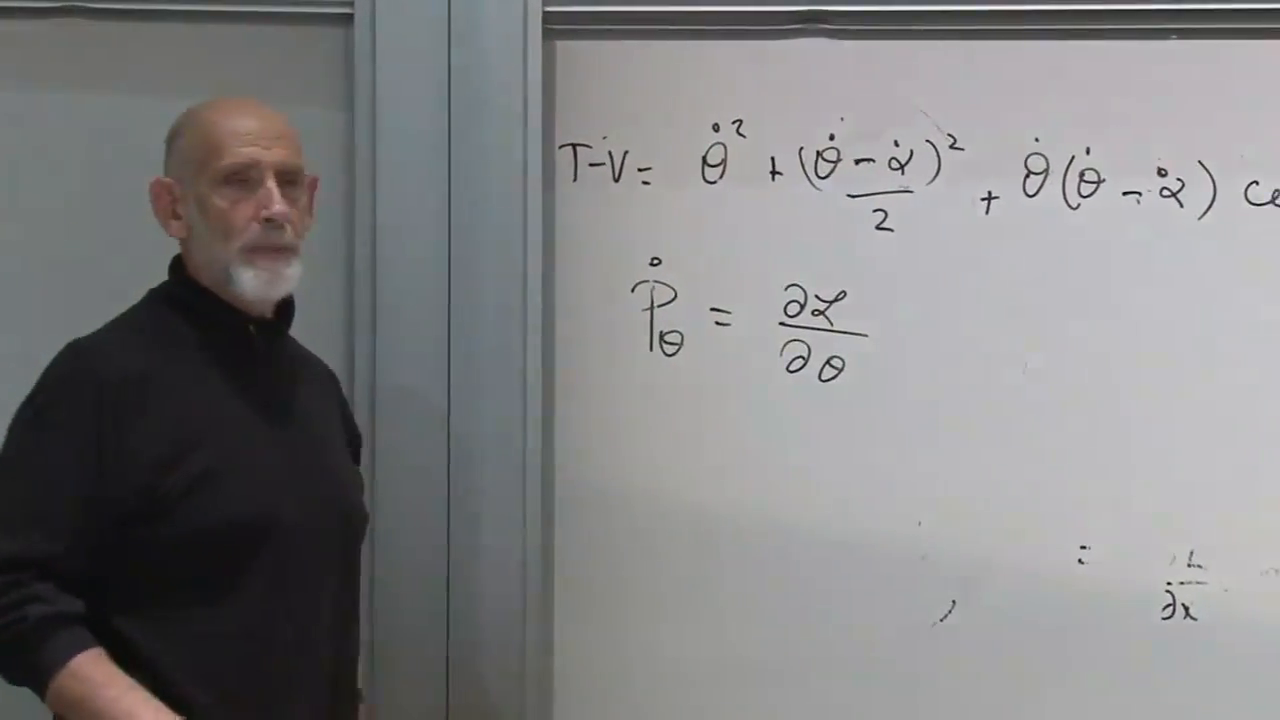
\includegraphics[width=0.84\textwidth]{lecture_06_figure_02.png}
  \caption{Вычисление для маятника без гравитации и
  \(\dot p_\theta=\partial L/\partial\theta\). Верхняя строка на доске сохраняет
  локальное обозначение с несогласованными знаками, обсуждавшееся в вопросе; нормализованная
  формула — уравнение ~\eqref{eq:l6-double-kinetic}.}
  \lectureframe{00:45:50}
\end{figure}

Как только известны \(T\) и \(V\), остальные уравнения получаются дифференцированием. Натяжения стержней и силы, обеспечивающие неизменность длин, вновь исчезли благодаря выбору координат.

\subsection{Что сохранение означает и чего не означает}

\begin{classroomqa} \audiencequestion{Можно ли непосредственно по уравнениям увидеть, хаотичен ли двойной маятник? \lecturetimestamp{00:44:57--00:45:25}} \lecturerresponse{Обычно нет, если просто смотреть на уравнения. При изменении параметров или энергии система может переходить от регулярного поведения к хаотическому. Здесь требуется больше структуры, чем дает непосредственный вид уравнений, и мы вернемся к этому позже.} \end{classroomqa}

\begin{classroomqa} \audiencequestion{В консервативной системе каждая ли \(\dot p_i\) равна нулю? \lecturetimestamp{00:45:25--00:46:24}} \lecturerresponse{Нет. Общее уравнение имеет вид \(\dot p_i=\partial L/\partial q_i\). Она обращается в нуль только тогда, когда \(q_i\) является циклической. Циклическая координата — это особенно простой случай, когда симметрия сдвигает одну координату, оставляя остальные фиксированными.} \end{classroomqa}

Если единственная цель — численно проследить эволюцию, неудобная система координат все равно годится; она лишь приводит к более длинным уравнениям. Выигрыш от удачного выбора носит концептуальный характер: сохраняющийся импульс виден еще до решения уравнений.

\begin{classroomqa} \audiencequestion{Без гравитации ведет ли себя двойной маятник так же просто, как один свободный маятник? \lecturetimestamp{00:47:02--00:47:35}} \lecturerresponse{Один свободный ротор вращается равномерно, потому что его единственный момент импульса полностью задает его движение. Двойной маятник может совершать очень сложное относительное движение, сохраняя при этом полный момент импульса. Если обе угловые скорости вначале равны нулю, система остается в покое; в противном случае две части взаимодействуют.} \end{classroomqa}

\begin{classroomqa} \audiencequestion{Являются ли \(\dot\theta\) и \(\dot\alpha\) по отдельности постоянными при отсутствии гравитации? \lecturetimestamp{00:47:36--00:52:42}} \lecturerresponse{Нет. Закон сохранения утверждает \(\dot p_\theta=0\), а не \(\ddot\theta=0\) или \(\ddot\alpha=0\). Выражение для \(p_\theta=\partial L/\partial\dot\theta\) содержит обе угловые скорости и зависит от \(\alpha\). Стержни передают моменты сил, позволяя двум грузам обмениваться моментом импульса и энергией. Это аналогично двум массам, соединенным пружиной: полный импульс и скорость центра масс постоянны, тогда как скорости каждой массы осциллируют. Вращательным аналогом здесь служит определенная коллективная комбинация, а не какой-либо из углов сам по себе.} \end{classroomqa}

\begin{classroomqa} \audiencequestion{Передаются ли через стержни силы, благодаря которым происходит обмен моментом импульса? \lecturetimestamp{00:52:43--00:53:34}} \lecturerresponse{Да. Сила, передаваемая вдоль стержня, не обязана проходить через точку подвеса другого звена, поэтому она может создавать момент силы. Момент силы — это просто вращательное действие силы, и здесь именно он приводит к ненулевым угловым ускорениям каждого звена.} \end{classroomqa}

\section{Гамильтониан как третья формулировка}

Гамильтониан — это энергия, но в этом состоит лишь его первое значение. Он также лежит в основе третьей формулировки механики. В уравнениях Ньютона используются силы и ускорения. Из принципа стационарного действия следуют уравнения Эйлера--Лагранжа. Для регулярных систем гамильтонова механика эквивалентна последним, но ее переменные и геометрия выглядят иначе.

Вместо \(q_i\) и \(\dot q_i\) используйте \(q_i\) и сопряженные с ними импульсы \(p_i\). Состояние системы с \(n\) степенями свободы требует \(2n\) чисел в любом из двух описаний: координат и скоростей либо координат и импульсов. Связь между ними задается соотношением: \begin{equation}
  p_i=\frac{\partial L}{\partial\dot q_i}.
  \label{eq:l6-legendre-map}
\end{equation} Когда эти соотношения можно обратить и выразить скорости как \(\dot q_i(q,p)\), определим \begin{equation}
  H(q,p)=\sum_i p_i\dot q_i-L(q,\dot q).
  \label{eq:l6-hamiltonian-definition}
\end{equation} Тогда скорости в правой части исключаются в пользу \(q\) и \(p\). Эта обратимость и есть предположение о регулярности преобразования Лежандра. Для сингулярных лагранжианов требуется более общая теория связей; этим элементарным построением они не охватываются.

\subsection{Обратимость до дифференциального исчисления}

Вспомним конечный набор абстрактных состояний, соединенных стрелками. Детерминистическое правило все же может оказаться необратимым, если два более ранних состояния переходят в одно более позднее. Будущее единственно, но прошлое — нет. Если обратить все стрелки, получится противоположный дефект: одно состояние ветвится в несколько будущих. На первой схеме стрелки сходятся, на второй — расходятся.

\begin{figure}[htbp] \centering
  \includegraphics[width=0.86\textwidth]{lecture_06_figure_11.png} \caption{Абстрактные отображения состояний, используемые для сопоставления обратимых циклов с запрещенными случаями схождения и расхождения.} \lectureframe{00:56:20} \end{figure}

Гамильтонов поток даст непрерывную версию этого утверждения. Облако точек фазового пространства может перемещаться и деформироваться, но не может приобрести сток, уничтожающий различия между состояниями, или источник, порождающий несколько будущих из одного состояния. Доказательство будет дано позже; пока эти диаграммы лишь мотивируют геометрию.

\begin{classroomqa} \audiencequestion{Следует ли понимать абстрактную диаграмму состояний как объект, движущийся в гравитационном поле? \lecturetimestamp{00:58:02--00:58:35}} \lecturerresponse{Нет. Точки — это всего лишь абстрактные состояния, а стрелки задают правило изменения состояния. Никакого пространственного или гравитационного смысла рисунку не приписывалось.} \end{classroomqa}

\begin{classroomqa} \audiencequestion{Чем запрещенное сходящееся отображение состояний отличается от черной дыры? \lecturetimestamp{00:58:40--00:59:28}} \lecturerresponse{Ответить можно лишь с трудом и большой осторожностью. Это уместный вопрос, но для правильного ответа требуется аккуратное описание полного состояния и его квантово-гравитационной эволюции. Элементарной диаграммы для этого недостаточно.} \end{classroomqa}

\section{Осциллятор в переменных, адаптированных к фазовому пространству}

Прежде чем выводить общие уравнения, рассмотрим гармонический осциллятор, записанный в специально подобранных переменных: \begin{equation}
  L=\frac{1}{2\omega}\dot q^2-\frac{\omega}{2}q^2.
  \label{eq:l6-rescaled-lagrangian}
\end{equation} Его сопряженный импульс равен \begin{equation}
  p=\frac{\partial L}{\partial\dot q}=\frac{\dot q}{\omega},
  \qquad
  \dot q=\omega p.
  \label{eq:l6-rescaled-momentum}
\end{equation} Подстановка в уравнение~\eqref{eq:l6-hamiltonian-definition} дает \begin{align}
  H&=p\dot q-L\\
   &=\omega p^2-\frac{\omega p^2}{2}+\frac{\omega q^2}{2}
    =\frac{\omega}{2}(p^2+q^2).
  \label{eq:l6-oscillator-hamiltonian}
\end{align}

\begin{figure}[htbp] \centering
  \includegraphics[width=0.86\textwidth]{lecture_06_figure_12.png} \caption{Преобразование Лежандра для адаптированного осциллятора и симметричный гамильтониан \(H=\tfrac{\omega}{2}(p^2+q^2)\).} \lectureframe{01:08:20} \end{figure}

Пространство переменных \(q\) и \(p\) — это фазовое пространство. Одна степень свободы дает двумерную плоскость; две степени свободы дают четырехмерное фазовое пространство. При фиксированной энергии осциллятора \begin{equation}
  p^2+q^2=\frac{2H}{\omega},
  \label{eq:l6-energy-circle}
\end{equation} поэтому траектория остается на окружности. Закон сохранения энергии ограничивает движение одной такой кривой.

\begin{figure}[htbp] \centering
  \includegraphics[width=0.82\textwidth]{lecture_06_figure_13.png} \caption{Вложенные окружности постоянной энергии на фазовой плоскости осциллятора: \(q\) по горизонтали, \(p\) по вертикали.} \lectureframe{01:13:20} \end{figure}

\section{Вывод уравнений Гамильтона}

Этот вывод — упражнение на дифференциал функции нескольких переменных. Для \(F(q,p)\) \begin{equation}
  \delta F=\sum_i\left(
  \frac{\partial F}{\partial q_i}\delta q_i
  +\frac{\partial F}{\partial p_i}\delta p_i\right).
  \label{eq:l6-total-differential}
\end{equation} Коэффициенты можно читать в обе стороны: коэффициент при \(\delta q_i\) равен \(\partial F/\partial q_i\), а коэффициент при \(\delta p_i\) равен \(\partial F/\partial p_i\).

Теперь проварьируем определяющее выражение для \(H\): \begin{align}
  \delta H
  &=\sum_i\left(\dot q_i\,\delta p_i
       +p_i\,\delta\dot q_i\right)-\delta L\\
  &=\sum_i\left(\dot q_i\,\delta p_i
       +p_i\,\delta\dot q_i
       -\frac{\partial L}{\partial q_i}\delta q_i
       -\frac{\partial L}{\partial\dot q_i}\delta\dot q_i\right).
  \label{eq:l6-vary-hamiltonian}
\end{align} Поскольку \(\partial L/\partial\dot q_i=p_i\), два члена с \(\delta\dot q_i\) сокращаются. Уравнения Эйлера--Лагранжа дают \(\partial L/\partial q_i=\dot p_i\), и остается \begin{equation}
  \delta H=\sum_i\left(\dot q_i\,\delta p_i
                     -\dot p_i\,\delta q_i\right).
  \label{eq:l6-reduced-variation}
\end{equation}

\begin{figure}[htbp] \centering
  \includegraphics[width=0.86\textwidth]{lecture_06_figure_14.png} \caption{Разложение \(\delta H\) по правилу произведения до сокращения членов \(p_i\,\delta\dot q_i\).} \lectureframe{01:18:40} \end{figure}

Сравнивая уравнение~\eqref{eq:l6-reduced-variation} с общим дифференциалом из уравнения~\eqref{eq:l6-total-differential}, из независимых коэффициентов получаем уравнения Гамильтона: \begin{equation}
  \boxed{
  \dot q_i=\frac{\partial H}{\partial p_i},
  \qquad
  \dot p_i=-\frac{\partial H}{\partial q_i}.}
  \label{eq:l6-hamilton-equations}
\end{equation}

\begin{figure}[htbp] \centering
  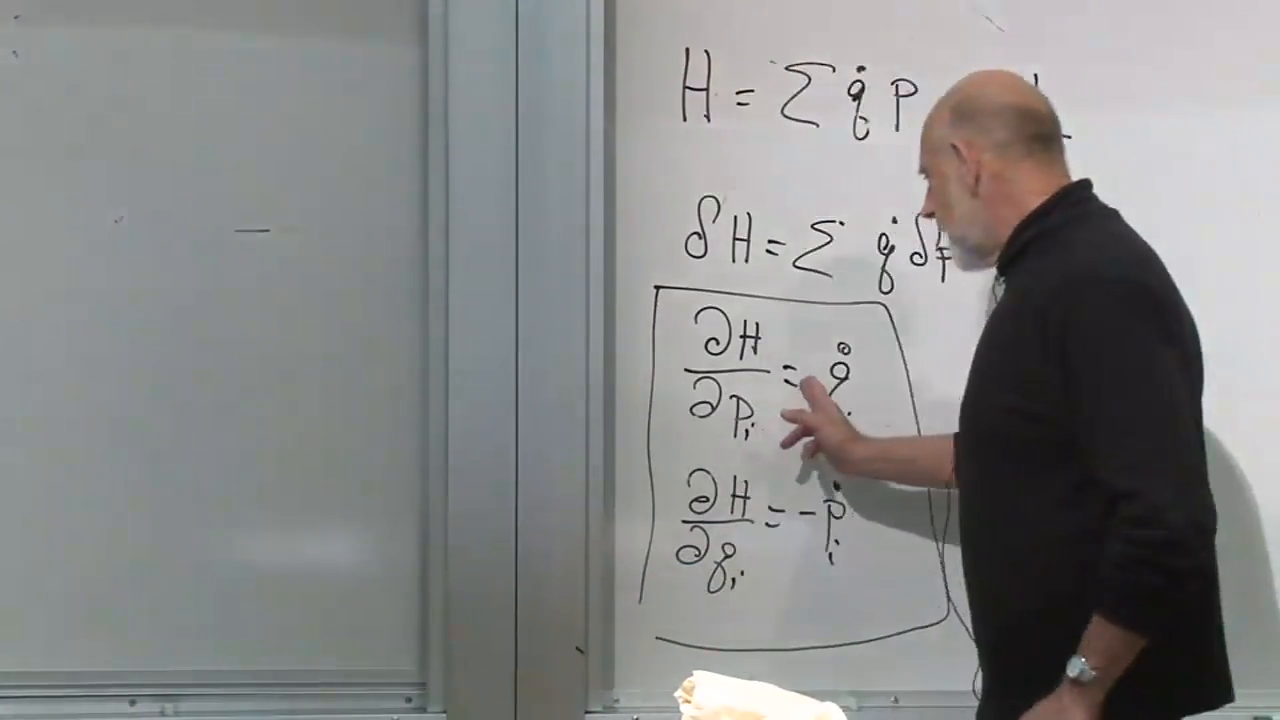
\includegraphics[width=0.78\textwidth]{lecture_06_figure_03.png} \caption{Определение гамильтониана, его вариация и выделенные в рамку канонические уравнения.} \lectureframe{01:22:18} \end{figure}

Для \(n\) координат это \(2n\) уравнений первого порядка. Формулировка Эйлера--Лагранжа, напротив, дает \(n\) уравнений второго порядка. Объем начальных данных и физическое содержание одинаковы.

\section{Движение осциллятора как жесткое вращение}

Применяя уравнения~\eqref{eq:l6-hamilton-equations} к уравнению~\eqref{eq:l6-oscillator-hamiltonian}, получаем \begin{equation}
  \dot q=\omega p,
  \qquad
  \dot p=-\omega q.
  \label{eq:l6-oscillator-first-order}
\end{equation} Дифференцируя первое уравнение и используя второе, \begin{equation}
  \ddot q=\omega\dot p=-\omega^2q.
  \label{eq:l6-oscillator-second-order}
\end{equation} Таким образом, эти два уравнения первого порядка в точности эквивалентны обычному уравнению осциллятора второго порядка вместе с определением импульса.

В фазовом пространстве вектор скорости в точке \((q,p)\) равен \((\dot q,\dot p)=(\omega p,-\omega q)\) и касателен к окружности постоянной энергии. Каждый радиус вращается с одной и той же угловой скоростью \(\omega\). Всю плоскость можно представить как жесткую вертушку или как несжимаемую фиктивную жидкость. Ее точки циркулируют; они не сжимаются в сток и не разлетаются от источника.

\begin{figure}[htbp] \centering
  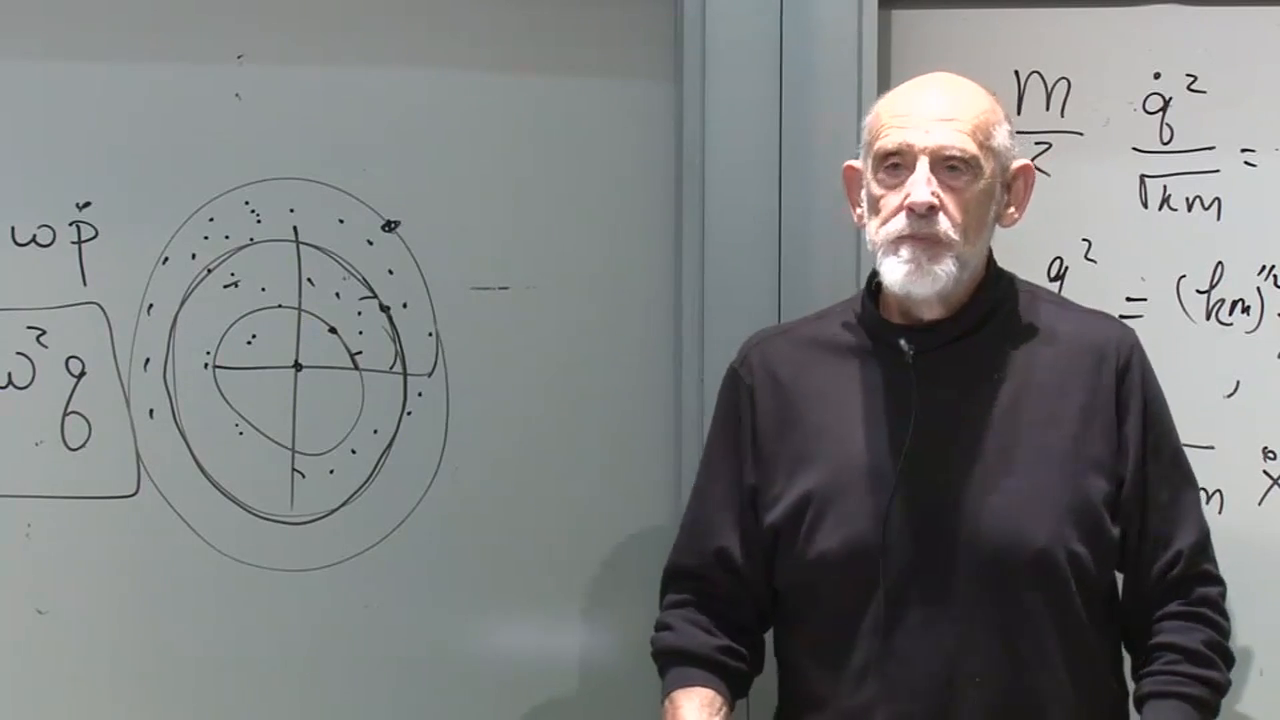
\includegraphics[width=0.86\textwidth]{lecture_06_figure_04.png} \caption{Облако начальных точек, распределенных по вложенным траекториям в фазовом пространстве. Гамильтонова эволюция перемещает это облако, а не схлопывает его в некоторое выделенное состояние.} \lectureframe{01:39:27} \end{figure}

\begin{figure}[htbp] \centering
  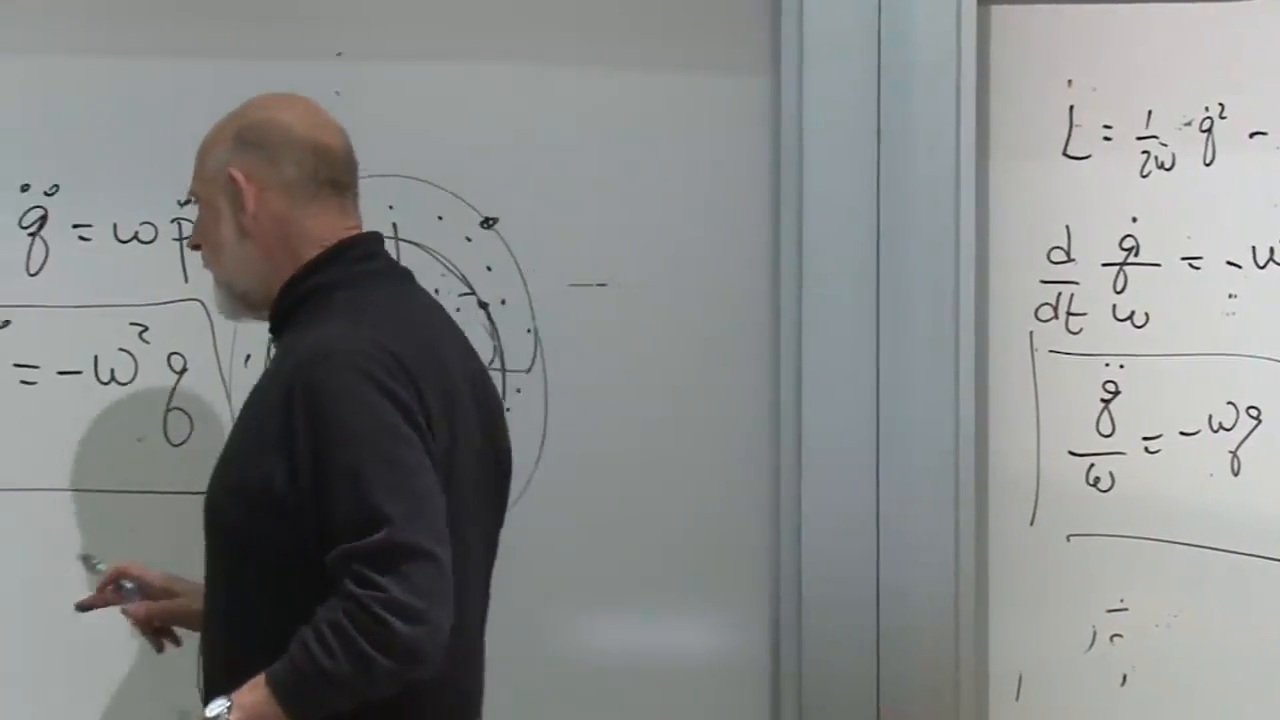
\includegraphics[width=0.90\textwidth]{lecture_06_figure_05.png} \caption{Фазовый портрет осциллятора рядом с эквивалентным уравнением Эйлера--Лагранжа \(\ddot q/\omega=-\omega q\).} \lectureframe{01:42:10} \end{figure}

Следующий шаг — превратить аналогию с жидкостью в теорему: гамильтонов поток не имеет локального схождения или расхождения. Этот результат вновь связывает непрерывную механику с обратимыми отображениями состояний, рассмотренными в начале курса.

\section{Вопросы, выявляющие выбор координат}

\begin{classroomqa}
  \audiencequestion{Является ли предположение о том, что скорости можно выразить через \(q\) и \(p\), теоремой или эмпирическим свойством физических систем?
  \lecturetimestamp{01:29:08--01:29:45}}
  \lecturerresponse{В рамках этого элементарного изложения это эмпирическая закономерность; более глубокая мотивация приходит из квантовой механики. Точнее, уравнение~\eqref{eq:l6-legendre-map} должно иметь невырожденный якобиан по скоростям. В современной механике встречаются и важные вырожденные лагранжианы, особенно системы со связями и калибровочные системы, но их гамильтонова формулировка требует дополнительного аппарата связей.}
\end{classroomqa}

Возражение, связанное с размерностями, объясняет, почему осциллятор был записан в непривычной форме уравнения~\eqref{eq:l6-rescaled-lagrangian}. Начнем вместо этого с обычной координаты \(x\):
\begin{equation}
  L=\frac{m}{2}\dot x^2-\frac{k}{2}x^2,
  \qquad
  \omega=\sqrt{\frac{k}{m}}.
  \label{eq:l6-ordinary-oscillator}
\end{equation}
Выберем
\begin{equation}
  q=(km)^{1/4}x.
  \label{eq:l6-oscillator-rescaling}
\end{equation}
Тогда \(q^2=\sqrt{km}\,x^2\) и \(\dot q^2=\sqrt{km}\,\dot x^2\), что в точности переводит уравнение~\eqref{eq:l6-ordinary-oscillator} в уравнение~\eqref{eq:l6-rescaled-lagrangian}. Новая \(q\) — это адаптированная обобщенная координата, а не длина, и сопряженная с ней \(p\) — не обычный механический импульс \(p_x=m\dot x\).

\begin{figure}[htbp]
  \centering
  \includegraphics[width=0.86\textwidth]{lecture_06_figure_15.png}
  \caption{Размерностное масштабирование от обычной координаты осциллятора \(x\) к адаптированной координате \(q=(km)^{1/4}x\).}
  \lectureframe{01:36:10}
\end{figure}

\begin{classroomqa}
  \audiencequestion{Как соотношение \(\omega p=\dot q\) может быть размерностно согласованным, и почему были выбраны эти переменные?
  \lecturetimestamp{01:29:46--01:39:22}}
  \lecturerresponse{Символ \(q\) не обязан иметь размерность длины, а сопряженный с ним \(p\) не обязан иметь размерность \(m\dot x\). Масштабирование в уравнении~\eqref{eq:l6-oscillator-rescaling} сохраняет размерность лагранжиана и заставляет \(q\) и \(p\) входить в \(H\) симметрично. В исходных переменных,
  \[
    H=\frac{p_x^2}{2m}+\frac{kx^2}{2},
  \]
  так что кривые постоянной энергии на плоскости \((x,p_x)\) являются эллипсами. На адаптированной плоскости \((q,p)\) это окружности. Масштабирование было выбрано, чтобы сделать эту симметрию наглядной.}
\end{classroomqa}

\begin{classroomqa}
  \audiencequestion{Как \(2n\) гамильтоновых уравнений первого порядка могут быть эквивалентны \(n\) уравнениям Лагранжа второго порядка?
  \lecturetimestamp{01:39:24--01:42:30}}
  \lecturerresponse{Для осциллятора продифференцируйте \(\dot q=\omega p\) и подставьте \(\dot p=-\omega q\); эта пара превращается в \(\ddot q=-\omega^2q\). Непосредственно из лагранжиана получаем
  \[
    \frac{d}{dt}\left(\frac{\dot q}{\omega}\right)
      =-\omega q,
  \]
  что и дает то же самое уравнение второго порядка. Одно из уравнений Гамильтона можно рассматривать как определение импульса через скорость, а другое описывает эволюцию этого импульса.}
\end{classroomqa}

\section{Почему важны фазовое пространство и потенциальная энергия}

\begin{classroomqa}
  \audiencequestion{Означает ли мощь гамильтониана, что фазовое пространство является лучшим геометрическим представлением, чем конфигурационное пространство?
  \lecturetimestamp{01:42:33--01:44:38}}
  \lecturerresponse{Они служат разным целям. Фазовое пространство делает циклы, поверхности постоянной энергии и отсутствие сходимости или расходимости необычайно наглядными. Конфигурационное пространство может быть лучше для других вопросов. Более глубокая причина того, что подчеркивается \(H\), состоит в том, что в квантовой механике — одной из современных тем, к которым направлено данное изложение механики, — он становится центральным и более интуитивным объектом.}
\end{classroomqa}

\begin{classroomqa}
  \audiencequestion{Следует ли рассматривать потенциальную энергию как интеграл силы?
  \lecturetimestamp{01:44:40--01:45:45}}
  \lecturerresponse{Для консервативных сил это утверждение верно с точностью до постоянной и с соответствующим знаком. Более полезно считать потенциал первичным и выводить из него обобщенную силу:
  \[
    F_i=-\frac{\partial V}{\partial q_i}.
  \]
  Именно этот член появляется в \(\dot p_i=\partial L/\partial q_i\), когда \(L=T-V\) и кинетическая энергия не зависит явно от \(q_i\).}
\end{classroomqa}

\begin{classroomqa}
  \audiencequestion{Какие проблемы переднего края призван прояснить этот путь к современной физике?
  \lecturetimestamp{01:45:46--01:47:47}}
  \lecturerresponse{Этот путь ведет к квантовой гравитации и космологии; физике элементарных частиц, включая сектор Хиггса и нейтрино; теории относительности; теории струн; и квантовой теории поля. Непреходящая теоретическая проблема состоит в том, чтобы объединить эти части в одну согласованную структуру, особенно квантовую механику с гравитацией и космологию с физикой частиц. Это было описание переднего края в том виде, в каком он виделся в 2011 году, а не утверждение, что его решение уже было известно.}
\end{classroomqa}

Два примера со связями и осциллятор теперь складываются в единую картину.
Обобщенные координаты устраняют ненужные силы. Симметрия выделяет сохраняющиеся канонические импульсы. Преобразование Лежандра заменяет скорости импульсами, а уравнения Гамильтона превращают динамику в поток на фазовом пространстве.
Для осциллятора этот поток представляет собой жесткое вращение; для произвольной системы геометрия этого потока придаст обратимому движению точный непрерывный смысл.
